\documentclass{amsart}

\usepackage[brazilian]{babel}
\usepackage[utf8]{inputenc}
\usepackage{graphicx}
\usepackage{mathtools}
\usepackage{amsthm}
\usepackage{thmtools,thm-restate}
\usepackage{amsfonts}
\usepackage{hyperref}
\usepackage[singlelinecheck=false]{caption}
\usepackage[backend=biber,url=true,doi=true,eprint=false,style=alphabetic]{biblatex}
\usepackage{enumitem}
\usepackage[justification=centering]{caption}
\usepackage{indentfirst}
\usepackage{algorithm}
\usepackage{algpseudocode}
\usepackage{listings}

\addbibresource{references.bib}

\makeatletter
\def\subsection{\@startsection{subsection}{3}%
  \z@{.5\linespacing\@plus.7\linespacing}{.1\linespacing}%
  {\normalfont\itshape}}
\makeatother

\DeclareMathOperator*{\argmin}{arg\,min}
\DeclareMathOperator*{\argmax}{arg\,max}

\newcommand\defeq{\mathrel{\overset{\makebox[0pt]{\mbox{\normalfont\tiny\sffamily def}}}{=}}}

\algrenewcommand\algorithmicrequire{\textbf{Input}}
\algrenewcommand\algorithmicensure{\textbf{Output}}

\captionsetup[table]{labelsep=space}

\theoremstyle{plain}

\newcounter{dummy-def}\numberwithin{dummy-def}{subsection}
\newtheorem{definition}[dummy-def]{Definição}
\newcounter{dummy-thm}\numberwithin{dummy-thm}{subsection}
\newtheorem{theorem}[dummy-thm]{Teorema}
\newcounter{dummy-prop}\numberwithin{dummy-prop}{subsection}
\newtheorem{proposition}[dummy-prop]{Proposição}
\newcounter{dummy-ex}\numberwithin{dummy-ex}{subsection}
\newtheorem{exercise}[dummy-ex]{Exercício}
\newcounter{dummy-eg}\numberwithin{dummy-eg}{subsection}
\newtheorem{example}[dummy-eg]{Exemplo}

\numberwithin{equation}{subsection}

\newcommand{\set}[1]{\mathbf{#1}}
\newcommand{\pr}{\mathbb{P}}
\renewcommand{\implies}{\Rightarrow}

\newcommand{\bigo}{\mathcal{O}}

\setlength{\parskip}{1em}

\lstset{frameround=fttt,
  language=[5.3]Lua,
	numbers=left,
	breaklines=true,
	keywordstyle=\bfseries,
	basicstyle=\ttfamily,
}

\newcommand{\code}[1]{\lstinline[mathescape=true]{#1}}
\newcommand{\mcode}[1]{\lstinline[mathescape]!#1!}


\title{%
  \noindent\rule{10cm}{0.8pt}\\
  Estudo sobre Sum-Product Networks e Aprendizagem Profunda\\[1ex]
  \scriptsize\mdseries
  PTC2669 - Introdução a Inteligência Computacional\\
  Instituto de Matemática e Estatística - USP\\%
  \noindent\rule{10cm}{0.8pt}
}
\xdef\shorttitle{Sum-Product Networks e Deep Learning - Renato Geh}
%\title[]{Estudo sobre Sum-Product Networks e Aprendizagem Profunda}
\author[]{Renato Lui Geh\\NUSP\@: 8536030}

\begin{document}

\begin{abstract}
  Modelos probabilísticos baseados em grafo (PGMs) são estruturas gráficas que representam
  compactamente uma distribuição de probabilidade. Raciocínio nestes modelos é, no caso geral,
  intratável e difícil. Um novo modelo proposto em 2011, Sum-Product Networks (SPNs), modela
  distribuições de forma que inferência é linear no número de arestas do grafo. SPNs têm tido
  grande atenção na área de Incerteza em Inteligência Artificial, já que experimentos empíricos têm
  mostrado grande vantagem em relação à outros modelos probabilísticos.

  Neste artigo, pretende-se mostrar a relação entre SPNs e o chamado \textit{Deep Learning}
  (Aprendizagem Profunda). \textit{Deep learning} tira proveito do uso de várias camadas ocultas de
  variáveis latentes para representar a distribuição de forma mais compacta, tornando raciocínio
  nestes modelos mais tratável. No entanto, aprendizagem profunda é extremamente complexo. SPNs são
  arquiteturas que tiram vantagem de camadas ocultas, podendo ser vistas como redes neurais
  probabilísticas. Esta próxima relação com redes neurais faz com que SPNs derivem o algoritmo de
  \textit{backpropagation} imediatamente.

  Na primeira parte deste documento, vamos introduzir algumas noções de probabilidade e argumentar
  o uso de Teoria de Probabilidade em raciocínio sob incerteza. Em seguida, serão apresentados
  alguns clássicos modelos probabilísticos baseados em grafo. Mostraremos como computar inferência
  e aprendizado em Redes Bayesianas (RBs) e em seguida discutiremos a relação entre RBs e SPNs e o
  porquê de usarmos SPNs. Apresentaremos a estrutura e propriedades fundamentais de SPNs e como
  realizar inferência. Discutiremos a questão de \textit{deep learning} em SPNs e mostraremos
  alguns algoritmos de aprendizagem. Ao final, teremos uma breve descrição das similaridades entre
  SPNs, PGMs e redes neurais artificiais.

  \vspace*{-2.5em}
\end{abstract}

\maketitle

\section{Introdução}

No começo da Inteligência Artificial (IA), acreditava-se que representação de conhecimento era
possível somente por meio de lógicas e outras técnicas neo-calculistas. De fato, o uso de lógicas é
atraente para a modelagem de conhecimento, já que sua semântica é natural ao racicínio humano e
computacionalmente tem bom desempenho. No entanto, quando queremos representar o mundo real, lógica
proposicional e de primeira ordem assumem contra-domínios binários e simplistas. Ou seja, eventos
no mundo ou sempre ocorrem ou nunca ocorrem. Por exemplo, considere a sentença

\begin{equation}\label{ave-voa}
  \text{Toda ave voa.}
\end{equation}

A princípio a sentença pode parecer verdadeira. Mas considere o caso de um avestruz, pinguim, emu
ou ornitorrinco, aves que são notórias por sua inabilidade aérea. E mesmo se a ave fosse conhecida
por voar, considere o caso em que sua asa está quebrada, ou que a ave esteja doente o suficiente
para não conseguir voar. Todos estes casos, por mais improváveis que sejam, são eventos que podem
de fato ocorrer. Uma solução para este problema é enumerarmos cada caso que a afirmação tenha
valoração diferente da sentença original. Porém, esta solução deve ser exaustiva para todos os
casos e inclusive pode haver um número infinito de exceções, por mais infinitamente improváveis que
sejam.

Este problema pode ser parcialmente resolvido (ou talvez até solucionado) por meio de graus de
crença, onde certas incertezas ou imprecisões podem ser descritas por meio de um intervalo
contínuo, por exemplo $[0,1]$. Esta formulação de conhecimento por meio da continualização de
eventos é chamada de Incerteza. Durante as décadas de 1960 até meados de 1980, pesquisadores da
área de Inteligência Artificial tentaram lidar com incertezas de diversas formas. Ferramentas como
lógica difusa e teoria de probabilidade foram elaboradas para tratar tais imprecisões. No entanto,
a comunidade de IA a princípio não recebeu teoria de probabilidade de forma receptiva. Não foi até
meados de 1980, que probabilidade ganhou destaque entre pesquisadores. Em~\cite{pearl-1988}, Judea
Pearl argumenta o porquê de se usar teoria de probabilidade para representar incerteza.

Podemos reformular a sentença~\ref{ave-voa}, através de probabilidades como

\begin{equation}
  \text{80\% das aves voam.}
\end{equation}

Onde os 20\% restantes são o resultado da somatória de todas as infinitas probabilidades que não
obedecem a regra original. Apesar de no mundo real esta probabilidade provavelmente não ser exata,
é uma abstração muito mais precisa que a usada em~\ref{ave-voa}.

\section{Noções de Teoria de Probabilidade}

Nesta seção iremos abordar conceitos básicos de teoria de probabilidade. Em específico, iremos
definir um modelo probabilístico, enumerar os axiomas de uma função de probabilidade e citar alguns
conceitos básicos como probabilidade condicional, regra da cadeia e regra de Bayes.

\subsection{Modelo probabilístico}

Denotaremos o conjunto de todos os subconjuntos de $\Omega$ como $2^\Omega$.

\begin{definition}\label{field-sets}
  Uma álgebra de conjuntos é um par $(\Omega,\mathcal{F})$, onde $\Omega$ é um conjunto e
  $\mathcal{F}$ é uma álgebra sob $\Omega$, ou seja, um conjunto não-vazio de todos os subconjuntos
  distintos de $\Omega$ fechados sobre complemento e união. Chamaremos os elementos de
  $\mathcal{F}$ de eventos e $\Omega$ de espaço de possibilidade.
\end{definition}

A partir do complemento e união, podemos aplicar De Morgan para provar que intersecção também é
fechada. Para exemplificar a definição~\ref{field-sets}, considere o espaço de possibilidades
$\Omega=\mathbb{Z}_2=\{0,1\}$. Então $(\Omega,\{\emptyset,\Omega\})$ e $(\Omega,\{\emptyset,\{0\},
\{1\},\Omega\})$ são álgebras de conjuntos. Note que $(\Omega,\{\emptyset,\Omega\})$ será sempre
uma álgebra de conjuntos. Da mesma forma, $(\Omega,2^\Omega)$ também é uma álgebra de conjuntos.

Esta definição de álgebra de conjuntos é suficiente para quando $\Omega$ é enumerável. No entanto,
isso restringe-nos a um domínio discreto. Neste artigo estudaremos apenas domínios discretos,
porém para definirmos para domínios contínuos, assumiríamos uma sigma-álgebra.

\begin{definition}
  Uma sigma-álgebra $\mathcal{A}$ é uma coleção de subconjuntos de $\Omega$ que contém $\Omega$ e
  é fechado sobre complemento e união de subconjuntos infinitamente enumeráveis.
\end{definition}

\begin{definition}\label{def:prob-model}
  Um modelo probabilístico, ou espaço de probabilidade, é uma tupla $(\Omega,\mathcal{F},\Pr)$,
  onde $\Omega$ é um conjunto finito de eventos atômicos, $(\Omega,\mathcal{F})$ é uma álgebra de
  conjuntos e $\Pr$ é uma função em $\mathcal{F}$ tal que:

  \begin{enumerate}
    \item $\Pr(\alpha)\geq 0$;
    \item $\Pr(\Omega)=1$;
    \item $\Pr(\alpha\cup\beta)=\Pr(\alpha)+\Pr(\beta)$, para eventos disjuntos $\alpha$ e $\beta$.
  \end{enumerate}
\end{definition}

As três regras enumeradas são os axiomas de probabilidade. Para exemplificar, considere o modelo
probabilístico que modela a distribuição de probabilidade de uma moeda viciada: $(\Omega=\{H, T\},
2^\Omega,\Pr)$. Se $H$ representa cara e $T$ coroa, então $\Pr(\emptyset)=0$, $\Pr(\{H\})=0.3$,
$\Pr(\{T\})=0.7$, $\Pr(\Omega)=1$.

Vamos enumerar algumas propriedades que são diretamente derivadas da
Definição~\ref{def:prob-model}.

\begin{restatable}[Complemento]{proposition}{complement}\label{prop:complement}
  Para qualquer evento $\alpha$, segue-se que $\Pr(\alpha)=1-\Pr(\alpha^c)$, onde $\alpha^c$ é o
  complemento de $\alpha$.
\end{restatable}

\begin{restatable}{proposition}{nullevent}\label{prop:nullevent}
  Seja $\Omega$ o evento de possibilidades e $\emptyset=\Omega^c$, então $\Pr(\emptyset)=0$.
\end{restatable}

\begin{restatable}[Monotonicidade]{proposition}{monotonicity}\label{prop:monotonicity}
  Sejam $\alpha$ e $\beta$ eventos. Se $\alpha\subseteq\beta$ então $\Pr(\alpha)\leq\Pr(\beta)$.
\end{restatable}

\begin{restatable}{proposition}{interval}\label{prop:interval}
  Para todo evento $\alpha$, temos que $0\leq\Pr(\alpha)\leq 1$.
\end{restatable}

\begin{restatable}{proposition}{union}\label{prop:union}
  Para quaisquer eventos $\alpha$ e $\beta$ (não necessariamente disjuntos), temos que $\Pr(\alpha
  \cup\beta)=\Pr(\alpha)+\Pr(\beta)+\Pr(\alpha\cap\beta)$.
\end{restatable}

\begin{restatable}{proposition}{superset}\label{prop:superset}
  Se $\Pr(\alpha)=1$ para algum evento arbitrário $\alpha$, então $\Pr(\beta)=\Pr(\alpha\cap\beta)$
  para qualquer evento $\beta$.
\end{restatable}

\subsection{Definições e proposições importantes}

A partir do modelo probabilístico definido na subseção anterior, vamos definir probabilidade
condicional.

\begin{definition}
  A probabilidade condicional $\Pr(\alpha|\beta)$ do evento $\alpha$ dado evento $\beta$ é dita por
  \begin{equation}
    \Pr(\alpha|\beta)=\frac{\Pr(\alpha\cap\beta)}{\Pr(\beta)}
  \end{equation}
  Quando $\Pr(\beta)=0$, a função não é definida. Por convenção, definiremos que
  $\Pr(\alpha|\beta)=0$ se $\Pr(\beta)=0$.
\end{definition}

A probabilidade condicional pode ser vista como uma atualização da crença do evento $\alpha$, já
que estamos interessados em saber a probabilidade do evento $\alpha$ dado que o evento $\beta$ já
foi dado (é conhecido). A partir da definição de probabilidade condicional, podemos derivar a regra
da cadeia.

Adotaremos uma notação mais simplificada com relação à operação de intersecção. Ao invés de
denotarmos uma probabilidade conjunta como $\Pr(\alpha\cap\beta)$, indicaremos a mesma
probabilidade como o equivalente $\Pr(\alpha,\beta)$. Semânticamente ambos são equivalentes.

\begin{restatable}[Regra da Cadeia]{proposition}{chainrule}\label{prop:chain-rule}
  Para qualquer sequência de eventos $\alpha_1,\ldots,\alpha_n$, temos que
  \begin{equation}
    \Pr(\alpha_1,\ldots,\alpha_n)=\Pr(\alpha_1)\prod_{i=1}^n \Pr(\alpha_i|\alpha_1,\ldots,
    \alpha_{i-1})
  \end{equation}
\end{restatable}

\begin{definition}
  Uma partição $\alpha_1,\ldots,\alpha_n$ de um espaço de possibilidades $\Omega$ é um conjunto
  onde $\bigcup_i \alpha_i=\Omega$ e $\alpha_i\cap\alpha_j=\emptyset$ para qualquer $i\neq j$ e
  $\alpha_i\neq\emptyset$.
\end{definition}

\begin{restatable}[Regra da Probabilidade Total]{proposition}{totalprob}\label{prop:total-prob}
  Dada uma partição $\alpha_1,\ldots,\alpha_n$ de $\Omega$, para qualquer evento $\beta$, segue-se
  que
  \begin{equation}
    \Pr(\beta)=\sum_{i=1}^n \Pr(\beta|\alpha_i)\Pr(\alpha_i)
  \end{equation}
\end{restatable}

\begin{restatable}[Regra de Bayes]{proposition}{bayesrule}\label{prop:bayes-rule}
  Sejam eventos $\alpha$ e $\beta$ com probabilidade positiva. Então
  \begin{equation*}
    \Pr(\beta|\alpha)=\frac{\Pr(\alpha|\beta)\Pr(\beta)}{\Pr(\alpha)}
  \end{equation*}
\end{restatable}

O que torna a Regra de Bayes um resultado importante é a possibilidade de se atualizar sua crença
em relação a uma condição. Por exemplo, considere o caso em que um médico busca saber a
probabilidade de um paciente ter contraído uma doença dados os sintomas. Na área médica, muitas
vezes é mais difícil encontrarmos a probabilidade dados os sintomas do que os sintomas dadas as
doenças, já que temos muitas vezes um certo determinismo quanto as probabilidades dos sintomas
ocorrerem em certas doenças (ex.:\ se o paciente tem gripe, então sabemos com probabilidade 1 que
ele apresentará coriza). Neste caso, podemos computar a probabilidade desejada pela regra de Bayes.

\subsection{Variáveis aleatórias}

\begin{definition}
  Uma variável aleatória é uma função $X:\Omega\to Val(X)$, onde $\Omega$ é um espaço de
  possibilidades e $Val(X)$ é o conjunto dos possíveis valores de $X$.
\end{definition}

Iremos abusar da notação e vamos considerar que a probabilidade de uma variável aleatória $X$ ter
um certo valor $x\in Val(X)$ será denotada como

\begin{equation*}
  \Pr(X=x) \coloneqq \Pr(\{w\in\Omega : X(w)=x\})
\end{equation*}

Variáveis aleatórias serão escritas como letras maiúsculas (ex.:\ $X$, $Y$, $Z$). Quando tratarmos
de valores de variáveis aleatórias usaremos letras minúsculas (ex.:\ $X=x$, $Y=y$, $Z=z$). Como
iremos tratar de casos discretos e finitos, $Val(X)$ é um conjunto finito. Trataremos
probabilidades de conjuntos de variáveis aleatórias da mesma forma, porém distinguiremos a notação
por meio do uso do negrito (ex.: $\mathbf{X}=\{X_1=x_1,\ldots,X_n=x_n\}$). Usaremos a notação

\begin{equation*}
  \Pr(\mathbf{X},\mathbf{Y}) \coloneqq \Pr(X_1,\ldots,X_n,Y_1,\ldots,Y_m)
\end{equation*}

Para representar a probabilidade conjunta das variáveis aleatórias em $\mathbf{X}$ e $\mathbf{Y}$.
Os resultados que encontramos para eventos atômicos (probabilidade condicional, regra de Bayes,
regra da probabilidade total, etc.) também valem para variáveis aleatórias e conjuntos de variáveis
aleatórias.

\begin{example}
  Considere que queremos criar um modelo probabilístico para descrever uma moeda. Vamos denotar por
  $C_1,\ldots,C_m$ as variáveis aleatórias que representam as jogadas. Para cada $C_i$,
  $Val(C_i)=\{cara,coroa\}$. A probabilidade conjunta de todas as jogadas é dada por $\Pr(C_1,
  \ldots,C_m)=\prod_{i=1}^m \Pr(C_i)$. Pela regra da probabilidade total, temos que a probabilidade
  de uma moeda $C_j$ ter um certo valor $c$ é dada por $\sum_{C_1,\ldots,C_{j-1},C_{j+1},C_n}
  \Pr(C_1,\ldots,C_j=c,\ldots,C_m)$, onde a somatória indica uma soma sob todos os valores
  de $C_i$ para $i\neq j$. Chamamos essa probabilidade de marginal e a soma de marginalização.
\end{example}

\section{Noções de Teoria de Grafos}

Apesar de ser possível criar modelos probabilísticos sem o uso de Teoria de Grafos, a utilização
destes não só torna mais visual e intuitivo o modelo, quanto proporciona uma maior facilidade
computacional, já que muitos problemas em grafos já foram solucionados ou otimizados, e portanto
constituem uma base forte para a construção de modelos.

Nesta seção iremos mostrar a definição de grafos e discutir algumas propriedades relevantes com o
que veremos mais adiante.

\subsection{Grafos direcionados e não-direcionados}

\begin{definition}
  Um grafo não-direcionado é uma tupla $G=(V,E)$, onde $V$ é o conjunto de vértices e $E$ é o
  conjunto de arestas em que cada elemento de $E$ é um par não-ordenado da forma $e_{ij}=(i,j)$,
  em que $i$ e $j$ são vértices em $V$. Em um grafo não-direcionado, $e_{ij}=e_{ji}$. Denotaremos
  $e_{ij}$ por $i-j$.
\end{definition}

\begin{definition}
  Um grafo direcionado (digrafo) é uma tupla $G=(V,E)$ onde $V$ é o conjunto de vértices e $E$ é o
  conjunto de arcos. Um elemento em $E$ é um par ordenado $e_{ij}=(i,j)\neq e_{ji}=(j,i)$. $e_{ij}$
  será representado como $i\to j$.
\end{definition}

Não distinguiremos os nomes arcos e arestas, nós e vértices. Ao invés disso diremos sempre aresta
e nó, independentemente da direção ou não-direção do grafo.

Por enquanto consideraremos apenas grafos direcionados. Contudo as propriedades que não citem
arestas direcionadas valem também para grafos não-direcionados.

Sejam $G=(V,E)$ um grafo direcionado e $X\in V$ um nó. O conjunto $Pa(X)$ é a coleção de ``pais''
de $X$. Um nó $Y\in V$ é pai de $X$ sse existe uma aresta direcionada $Y\to X$. X é então filho de
$Y$. Os vizinhos de $X$ são denotados pelo conjunto $Ne(X)$, onde $Ne(X)=\{\forall v\in V : e_{x,v}
\vee e_{v,x}\}$. Um caminho é uma sequência de vértices $v_1,\ldots,v_m$ tal que exista uma aresta
$e_{v_i,v_j}$ para $i\leq j$. Um ciclo é um caminho $v_i,\ldots,v_j$ onde $i=j$. Um digrafo
acíclico (DAG) é um digrafo que não possui ciclos. O conjunto $De(X)$ de descendentes de $X$ é um
subgrafo de $G$ em que não há ciclos e que possui um caminho $\forall Y\in De(X), X\to Y$. O
conjunto $An(X)$ de ancestrais de $X$ é o subgrafo acíclico em que haja um caminho $\forall Y\in
An(X), Y\to X$. O conjunto $Nd(X)$ é $V\setminus De(X)$. Uma ordenação topológica dos vértices de
um grafo acíclico é uma ordenação onde os índices dos vértices $v_i$ e $v_j$ são tal que $i<j$ sse
$v_j\not\in An(v_i)$.

\section{Modelos Probabilísticos Clássicos Baseados em Grafo}

Chamamos de Modelos Probabilísticos Baseados em Grafo (PGMs -- Probabilistic Graphical Models) um
modelo probabilístico que tenha sua distribuição de probabilidade representada compactamente por um
grafo. Queremos representar a distribuição de forma compacta devido ao tamanho exponencial de
termos que uma distribuição de probabilidade expressa. Uma distribuição de probabilidade com $n$
variáveis e $p = \max |Val(X_i)|$ tem um número total de probabilidades e instanciações
$\bigo(p^n)$. Portanto, lidar diretamente com a distribuição é intratável no caso geral. Podemos
representar a distribuição de forma compacta assumindo (in)dependências entre eventos.

Adotamos a nomenclatura descrita em~\cite{peharz-spn} e consideraremos como PGMs clássicos (CPGMs)
os modelos de Redes Bayesianas e Redes de Markov. Nesta seção descreveremos Redes Bayesianas (RBs)
e mencionaremos brevemente Redes de Markov (RMs) afim de posteriormente compararmos as semelhanças
e diferenças entre SPNs e CPGMs.

\subsection{D-separação}

Podemos representar (in)dependências entre eventos (ou variáveis) por meio de um DAG\@. Dizemos que
$X$ depende de $Y$ se $X$ e $Y$ estão diretamente correlacionados, ou seja, são probabilisticamente
dependentes. Vamos representar esta dependência por meio de uma aresta

\begin{figure}[h]
  \centering{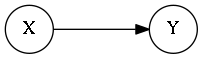
\includegraphics[scale=0.3]{imgs/d-sep1.png}}
  \caption{Um grafo de dependência onde os nós $X$ e $Y$ são probabilisticamente dependentes. Neste
  caso temos que $X\perp Y$.}
\end{figure}

que representa uma relação $X\not\perp Y$: $X$ é dependente de $Y$. O grafo que representa estas
relações entre variáveis é chamado de grafo de dependência. Podemos resumir as relações de
dependência em um grafo de dependência em três casos:

\begin{figure}[h]
  \centering{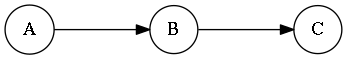
\includegraphics[scale=0.3]{imgs/d-sep2.png}}
  \caption{Em uma conexão serial temos que $A\perp C|B$ e $A\not\perp C|\emptyset$.}\label{serial-connection}
\end{figure}

O grafo descrito na Figura~\ref{serial-connection} é chamado de \textit{conexão serial}. O nó $B$
bloqueia nós $A$ e $C$, o que resulta em $A$ e $C$ serem somente independentes um do outro (ou
seja, não há aresta de dependência) se $B$ for removido. Portanto, podemos dizer que $A\perp C|B$ e
$A\not\perp C|\emptyset$. Em outras palavras, $A$ e $C$ estarão desbloqueados se removermos $B$.
Senão, eles estarão bloqueados por $B$.  Dizemos então que $A$ e $C$ são \textit{d-separados} por
$B$.

O segundo caso é conhecido como \textit{conexão divergente}, e ocorre quando um nó tem duas arestas
que conectam diretamente dois outros nós distintos. Podemos ver $B$ como uma causa em comum dos
efeitos $A$ e $C$.

\begin{figure}[h]
  \centering{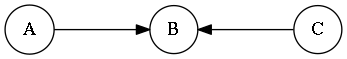
\includegraphics[scale=0.3]{imgs/d-sep3.png}}
  \caption{Em uma conexão divergente, temos que $A\perp C|B$ e $A\not\perp C|\emptyset$.}\label{divergent-connection}
\end{figure}

Note que se aplicarmos o que foi dito anteriormente sobre conexões seriais, podemos chegar as
mesmas conlusões. Se removermos o nó $B$, temos que $A$ e $C$ estarão desbloqueados e portanto
tornarão-se dependentes $A\not\perp C|\emptyset$. Se não removermos, $B$ bloqueia $A$ e $C$ e
então $A\perp C|B$. Conclue-se que $A$ e $C$ são d-separados por $B$.

O terceiro e último caso é chamado de \textit{conexão convergente}. Neste caso temos que $B$ é um
efeito em comum de $A$ e $C$ (ou $A$ e $C$ são uma causa em comum de $B$). Essa situação também é
chamada de \textit{explaining away}.

\begin{figure}[h]
  \centering{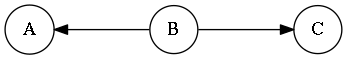
\includegraphics[scale=0.3]{imgs/d-sep4.png}}
  \caption{Em uma conexão convergente, temos que $A\not\perp C|B$ e $A\perp C|\emptyset$.}\label{convergent-connection}
\end{figure}

A trilha de $A$ para $C$ está desbloqueada quando $B$ não é removido e bloqueada quando $B$ é
removido. O nó $A$ é independente de $C$ quando não temos efeitos em comum e são dependentes entre
si quando há um efeito em comum. Neste caso dizemos que $A$ e $C$ são d-conectados por $B$. Apesar
de contra-intuitivo a primeira vista, tome o seguinte exemplo:

\begin{example}
  \begin{figure}[h]
    \centering{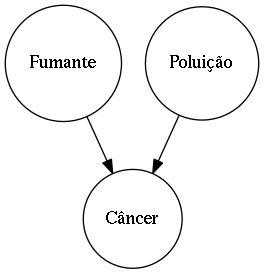
\includegraphics[scale=0.3]{imgs/d-sep5.png}}
    \caption{\textit{Fumante} e \textit{Poluição} são inicialmente independentes entre si. No
    entanto, quando soubermos que nosso paciente tem \textit{Câncer}, pode ser que tenhamos que
    alterar as probabilidades de nossas causas de acordo com o observado.}
  \end{figure}

  Considere a situação em que temos um grafo de dependência que atribue \textit{Fumante} e
  \textit{Poluição} como causas comuns ao efeito \textit{Câncer}. Consideraremos que o paciente
  fumar e este viver em um ambiente poluído são dois eventos independentes (se assumirmos que fumar
  não leva a poluição e que pessoas que fumam não tendem a viver em ambientes poluídos) e que fumar
  e poluição causam câncer (estamos simplificando o mundo para adequar-se ao nosso exemplo). Mas
  suponha que nosso paciente tem câncer. Então podemos dizer que a probabilidade dele fumar ou
  estar em constante presença com poluição aumenta, já que ambas são causas de câncer. Se então
  descobrirmos que nosso paciente fuma, isso pode levar a diminuição de nossa crença de que ele
  esteve em contato com poluição, já que acabamos de achar uma provável causa para o câncer do
  paciente. Note que mesmo que duas causas sejam independentes entre si separadamente (se não
  considerarmos a variável \textit{Câncer}), elas terão uma influência direta entre si quando
  conhecermos o efeito em comum.
\end{example}

Antes de definirmos d-separação, vamos definir o conceito de trilha bloqueada ou desbloqueada.

\begin{definition}
  Uma trilha de $X$ para $Y$ é bloqueada por um conjunto de nós $\mathcal{B}$ se
  \begin{enumerate}
    \item $X$ ou $Y$ pertencem a $\mathcal{B}$, ou
    \item Existe uma conexão serial ou divergente $X,Y,Z$ e $Y\in\mathcal{B}$, ou
    \item Existe uma conexão convergente $X\to Y\gets Z$ e $(\{Y\}\cup Nd(Y))\not\subseteq
      \mathcal{B}$, ou seja, nem $Y$ nem qualquer outro descendente de $Y$ pertencem a
      $\mathcal{B}$.
  \end{enumerate}
\end{definition}

\begin{definition}
  Os conjuntos de nós $\set{X}$ e $\set{Y}$ são d-separados por um conjunto de nós $\set{Z}$ se
  toda trilha de uma variável $X\in\set{X}$ para uma variável $Y\in\set{Y}$ está bloqueada por $Z$.
  Senão, $\set{X}$ e $\set{Y}$ são d-conectados. Vamos denotar d-separação pelo símbolo $\perp_d$.
  Portanto, se $\set{X}$ e $\set{Y}$ estão d-separados por $\set{Z}$

  \begin{equation*}
    \set{X}\perp_d\set{Y}|\set{Z}
  \end{equation*}
\end{definition}

Em outras palavras, d-separação indica independência.

\subsection{Redes Bayesianas}

Uma Rede Bayesiana é um modelo probabilístico que busca representar uma distribuição de
probabilidade de forma compacta por meio de um grafo.

\begin{definition}
  Uma Rede Bayesiana $\mathcal{N}$ é uma tupla $\mathcal{N}=(\Omega,\mathcal{F},\Pr,G)$, onde
  $\Omega$ é o espaço de possibilidades, $\mathcal{F}$ é uma álgebra sobre $\Omega$, $\Pr$ é uma
  função de probabilidade e $G=(\set{X},E)$ é um grafo onde $\set{X}$ é o conjunto de variáveis
  aleatórias de $\mathcal{N}$ e $E$ é o conjunto de arestas. Cada variável aleatória
  $X_i\in\set{X}$ representa uma probabilidade condicional $\Pr(X_i|Pa(X_i)$. Uma Rede Bayesiana é
  uma representação para a distribuição de probabilidade conjunta

  \begin{equation*}
    \Pr(\set{X}=\{X_1,\ldots,X_n\})=\prod_{X\in\set{X}} \Pr(X|Pa(X))
  \end{equation*}
\end{definition}



%--------------------------------------------------------------------------------------------------

\newpage
\appendix
\section{Provas}

\complement*
\begin{proof}
  Seja $\Omega$ o espaço de possibilidades em que $\alpha$ está contido. Como $\alpha$ e $\alpha^c$
  são conjuntos disjuntos e exaustivos em $\Omega$, então segue-se do axioma $\Pr(\Omega)=1$ que
  $\Pr(\alpha)+\Pr(\alpha^c)=\Pr(\Omega)=1$. Portanto temos que $\Pr(\alpha)=1-\Pr(\alpha^c)$.
\end{proof}

\nullevent*
\begin{proof}
  Assuma que $\Pr(\emptyset)>0$. Pelo axioma da probabilidade, temos que $\Pr(\alpha\cup\beta)=
  \Pr(\alpha)+\Pr(\beta)$ se $\alpha$ e $\beta$ são disjuntos. Então $\Pr(\emptyset\cup\emptyset)=
  \Pr(\emptyset)+\Pr(\emptyset)$, já que um conjunto vazio é disjunto consigo próprio. Mas
  $\emptyset\cup\emptyset=\emptyset$, portanto $\Pr(\emptyset)=2\Pr(\emptyset)$, o que é uma
  contradição se $\Pr(\emptyset)>0$. Pelo primeiro axioma, $\Pr(\emptyset)=0$.
\end{proof}

\monotonicity*
\begin{proof}
  Assuma que $\Pr(\alpha)>\Pr(\beta)$ quando $\alpha\subseteq\beta$. Agora considere $\alpha=
  \emptyset$; $\Pr(\emptyset)>\Pr(\beta)$. Mas $\Pr(\emptyset)=0\implies 0>\Pr(\beta)$, e pelo
  axioma da probabilidade, $\Pr(\beta)\geq 0$, o que é uma contradição. Portanto $\Pr(\alpha)\geq
  \Pr(\beta)$.
\end{proof}

\interval*
\begin{proof}
  Pelo primeiro axioma da probabilidade, temos que $\Pr(\alpha)\geq 0$. Considere $\Pr(\alpha)>1$.
  Como $\Pr(\alpha)=1-\Pr(\alpha^c)$ então $\Pr(\alpha^c)<0$, o que contradiz o primeiro axioma.
  Portanto, $0\leq\Pr(\alpha)\leq 1$.
\end{proof}

\union*
\begin{proof}
  Pelo terceiro axioma, $\Pr(\beta)=\Pr(\alpha\cap\beta)+\Pr(\beta\setminus(\alpha\cap\beta))$,
  onde $\alpha\cap\beta$ e $\beta\setminus(\alpha\cap\beta)$ são disjuntos. O terceiro axioma,
  $\Pr(\bigcup_i X_i)=\sum_i\Pr(X_i)$ é para conjuntos disjuntos. Portanto: $\Pr(\alpha\cup(\beta
  \setminus(\alpha\cap\beta)))=\Pr(\alpha)+\Pr(\beta\setminus(\alpha\cap\beta))$. Substituindo
  $\Pr(\beta\setminus(\alpha\cap\beta))$ por $\Pr(\beta)-\Pr(\alpha\cap\beta)$, $\Pr(\alpha\cup(
  \beta\setminus(\alpha\cap\beta)))=\Pr(\alpha)+\Pr(\beta)-\Pr(\alpha\cap\beta)$. Mas $\alpha\cup(
  \beta\setminus(\alpha\cap\beta))=\alpha\cup\beta$, então $\Pr(\alpha\cup\beta)=\Pr(\alpha)+\Pr(
  \beta)-\Pr(\alpha\cap\beta)$.
\end{proof}

\superset*
\begin{proof}
  $\Pr(\alpha\cup\beta)=\Pr(\alpha)+\Pr(\beta)-\Pr(\alpha\cap\beta)$. Como $\Pr(\alpha)=1$ e se
  $\alpha$ acontece com certeza então $\Pr(\alpha\cup\beta)=\Pr(\Omega)=1$, então $1=1+\Pr(\beta)-
  \Pr(\alpha\cap\beta)\implies\Pr(\beta)=\Pr(\alpha\cap\beta)$.
\end{proof}

\chainrule*
\begin{proof}
  Vamos provar por indução. Para a base $n=2$ temos diretamente da definição de probabilidade
  condicional que:

  \begin{equation*}
    \Pr(\alpha_2|\alpha_1)=\frac{\Pr(\alpha_1,\alpha_2)}{\Pr(\alpha_1)}\Rightarrow\Pr(\alpha_1
    ,\alpha_2)=\Pr(\alpha_1)\Pr(\alpha_2|\alpha_1)
  \end{equation*}

  Para o $k$-ésimo caso:

  \begin{equation*}
    \Pr(\alpha_k|\alpha_1,\ldots,\alpha_{k-1})=\frac{\Pr(\alpha_1,\ldots,\alpha_k)}
    {\Pr(\alpha_1,\ldots,\alpha_{k-1})}
  \end{equation*}

  \begin{equation}\label{chainrule:1}
    \Pr(\alpha_1,\ldots,\alpha_k)=\Pr(\alpha_1,\ldots,\alpha_{k-1})
      \Pr(\alpha_k|\alpha_1,\ldots,\alpha_{k-1})
  \end{equation}

  Mas $\Pr(\alpha_1,\ldots,\alpha_{k-1})$ pode ser transformado em

  \begin{equation}\label{chainrule:2}
    \Pr(\alpha_1,\ldots,\alpha_{k-1})=\Pr(\alpha_1,\ldots,\alpha_{k-2})
      \Pr(\alpha_{k-1}|\alpha_1,\ldots,\alpha_{k-2})
  \end{equation}

  Aplicando~\ref{chainrule:2} em~\ref{chainrule:1} temos que

  \begin{equation*}
    \Pr(\alpha_1,\ldots,\alpha_k)=\Pr(\alpha_1,\ldots,\alpha_{k-2})\Pr(\alpha_{k-1}|
      \alpha_1,\ldots,\alpha_{k-2})\Pr(\alpha_k|\alpha_1,\ldots,\alpha_{k-1})
  \end{equation*}

  Para o $(k+1)$-ésimo caso

  \begin{equation*}
    \Pr(\alpha_{k+1}|\alpha_1,\ldots,\alpha_k)=\frac{\Pr(\alpha_1,\ldots,\alpha_{k+1})}
      {\Pr(\alpha_1,\ldots,\alpha_k)}
  \end{equation*}

  \begin{equation*}
    \Pr(\alpha_1,\ldots,\alpha_{k+1})=\Pr(\alpha_1,\ldots,\alpha_k)\Pr(\alpha_{k+1}|
      \alpha_1,\ldots,\alpha_k)
  \end{equation*}

  Pela hipótese de indução $\Pr(\alpha_1,\ldots,\alpha_k)$. Portanto, para $n\geq2$ temos

  \begin{align*}
    \Pr(\alpha_1,\ldots,\alpha_n)&=\Pr(\alpha_1)\Pr(\alpha_2|\alpha_1)\ldots\Pr(\alpha_n|
      \alpha_1,\ldots,\alpha_{n-1})\\
      &=\Pr(\alpha_1)\prod_{i=2}^n\Pr(\alpha_i|\alpha_1,\ldots,\alpha_{i-1})
  \end{align*}
\end{proof}

\totalprob*
\begin{proof}
  Como $\alpha_1,\ldots,\alpha_n$ é disjunto pela definição de partição, então
  \begin{equation}\label{totalprob:1}
    \Pr(\beta\cap(\bigcup_i \alpha_i))=\Pr((\beta\cap\alpha_1)\cup\ldots\cup(\beta\cap\alpha_n))
  \end{equation}
  Pela definição de probabilidade condicional, para um $i$ arbitrário, temos que
  \begin{equation}\label{totalprob:2}
    \Pr(\beta|\alpha_i)=\frac{\Pr(\beta\cap\alpha_i)}{\Pr(\alpha_i)}\implies\Pr(\beta\cap\alpha_i)=
    \Pr(\beta|\alpha_i)\Pr(\alpha_i)
  \end{equation}
  Aplicando-se~\ref{totalprob:2} em~\ref{totalprob:1}
  \begin{equation*}
    \Pr(\beta\cap(\bigcup_i \alpha_i))=\Pr(\beta|\alpha_1)\Pr(\alpha_1)+\cdots+\Pr(\beta|\alpha_n)
    \Pr(\alpha_n)
  \end{equation*}
  Como $\alpha_1,\ldots,\alpha_n$ é disjunto e exaustivo em $\Omega$, então $\beta\cap(\alpha_1\cup
  \ldots\cup\alpha_n)=\beta\cap\Omega=\beta$. Portanto
  \begin{equation*}
    \Pr(\beta)=\sum_i \Pr(\beta|\alpha_i)\Pr(\alpha_i)
  \end{equation*}
\end{proof}

\bayesrule*
\begin{proof}
  Pela definição de probabilidade condicional
  \begin{equation}\label{bayesrule:1}
    \Pr(\beta|\alpha)=\frac{\Pr(\alpha,\beta)}{\Pr(\alpha)}\implies\Pr(\alpha,\beta)=\Pr(\beta|
    \alpha)\Pr(\alpha)
  \end{equation}
  Aplicando-se~\ref{bayesrule:1} em $\Pr(\alpha|\beta)$
  \begin{equation*}
    \Pr(\alpha|\beta)=\frac{\Pr(\alpha,\beta)}{\Pr(\beta)}\implies\Pr(\alpha|\beta)=\frac{\Pr(
    \beta|\alpha)\Pr(\alpha)}{\Pr(\beta)}
  \end{equation*}
\end{proof}

\newpage

\printbibliography[]

\end{document}
